%%% Parámetros %%%

\begin{frame}{Experimentos y evaluación}{Parámetros}
\begin{itemize}
\item Monitor de carga
\begin{itemize}
	\item $T_m = 1seg$
\end{itemize}
\item Algoritmo reactivo
\begin{itemize}
	\item $\omega = 1$ réplica
\end{itemize} 
\item Algoritmo predictivo 
\begin{itemize}
	\item $\theta = 5$ réplicas
	\item $n = 100$ muestras
	\item $\beta = 0.25$
\end{itemize} 
\item Administrador de réplicas
\begin{itemize}
	\item Ventana de tiempo de ejecución
	\begin{itemize}
		\item $T_r = 5seg$
		\item $T_p = 100seg$
	\end{itemize}
	\item $\beta = 2$ alertas consecutivas
\end{itemize} 
\end{itemize}
\end{frame}

%%% App 1 - Constante %%%

\begin{frame}{Experimentos y evaluación}{Aplicación 1 - Constante - Rendimiento y cantidad de réplicas}

\begin{itemize}
\item 96 eventos/segundo con uso del modelo \textit{vs} 16 eventos/segundo sin uso del modelo
\item Mejora de 5 veces más eventos/segundo
\end{itemize}

\begin{multicols}{2}
\begin{figure}[p]
	\centering
	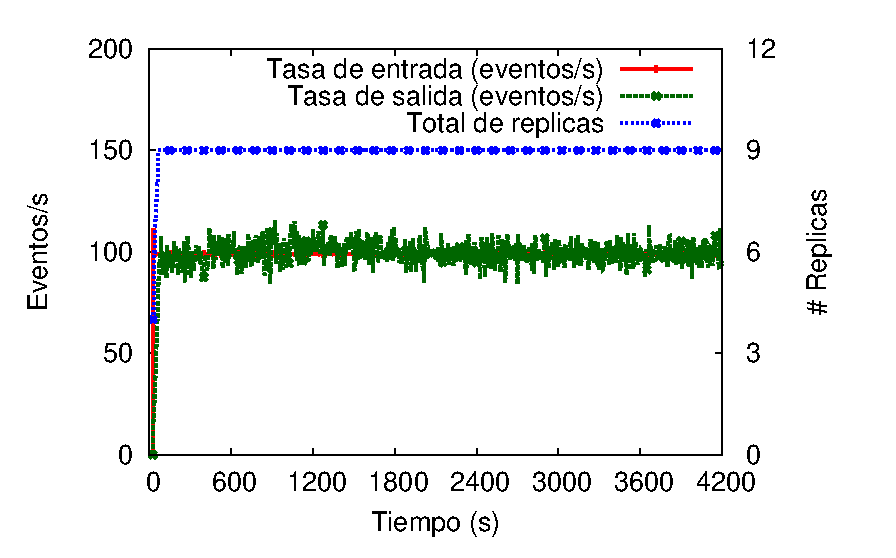
\includegraphics[scale=0.4]{images/exp/app1/uniform/cm/processSystem.eps}
\end{figure}

\begin{figure}[p]
	\centering
	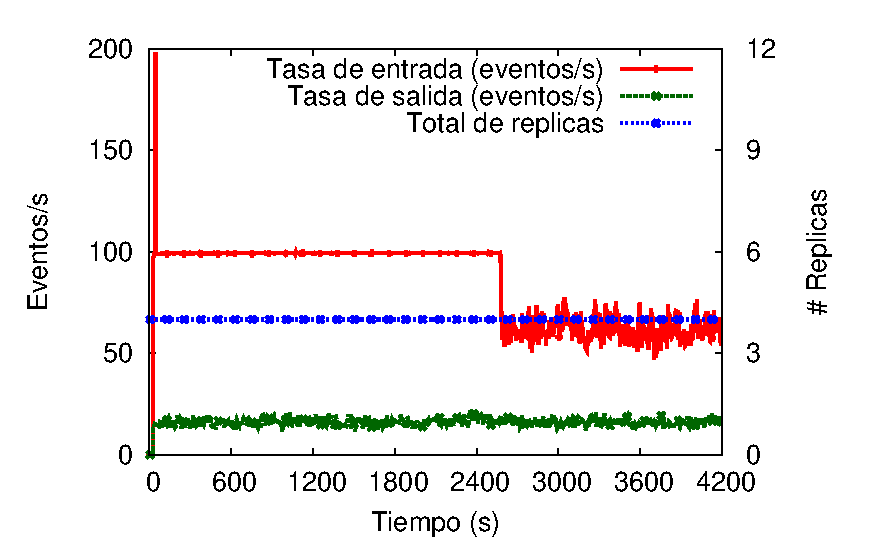
\includegraphics[scale=0.4]{images/exp/app1/uniform/sm/processSystem.eps}
\end{figure}
\end{multicols}
\end{frame}

\begin{frame}{Experimentos y evaluación}{Aplicación 1 - Constante - Cantidad total de eventos procesados}

\begin{itemize}
\item 401.618 eventos procesados con uso del modelo \textit{vs} 67.141 eventos procesados sin uso del modelo
\item Mejora de 6 veces la cantidad de eventos procesados
\end{itemize}

\begin{multicols}{2}
\begin{figure}[p]
	\centering
	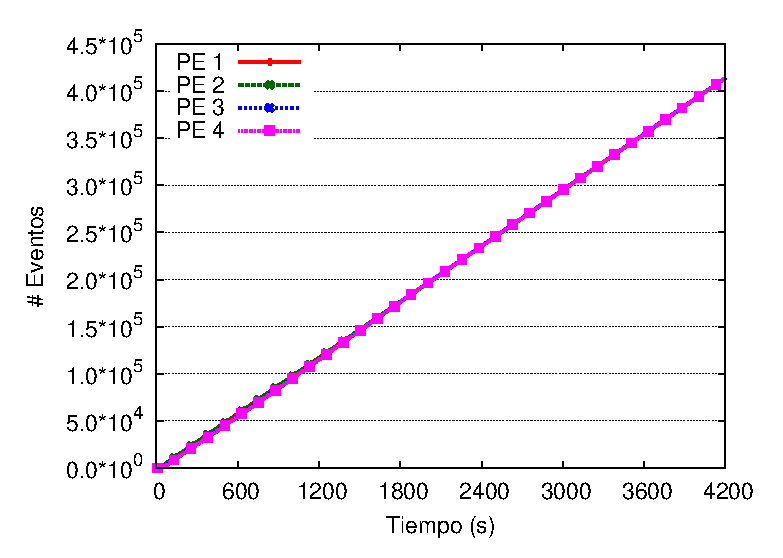
\includegraphics[scale=0.475]{images/exp/app1/uniform/cm/eventCount.eps}
\end{figure}

\begin{figure}[p]
	\centering
	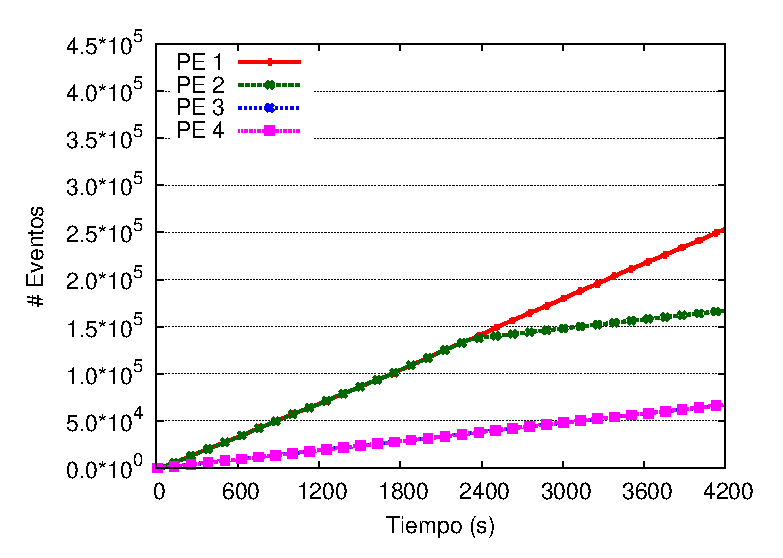
\includegraphics[scale=0.475]{images/exp/app1/uniform/sm/eventCount.eps}
\end{figure}
\end{multicols}
\end{frame}

%%% App 1 - Variable %%%

\begin{frame}{Experimentos y evaluación}{Aplicación 1 - Variable - Rendimiento y cantidad de réplicas}

\begin{itemize}
\item 72 eventos/segundo con uso del modelo \textit{vs} 19 eventos/segundo sin uso del modelo
\item Mejora de 3 veces más eventos/segundo
\end{itemize}

\begin{multicols}{2}
\begin{figure}[p]
	\centering
	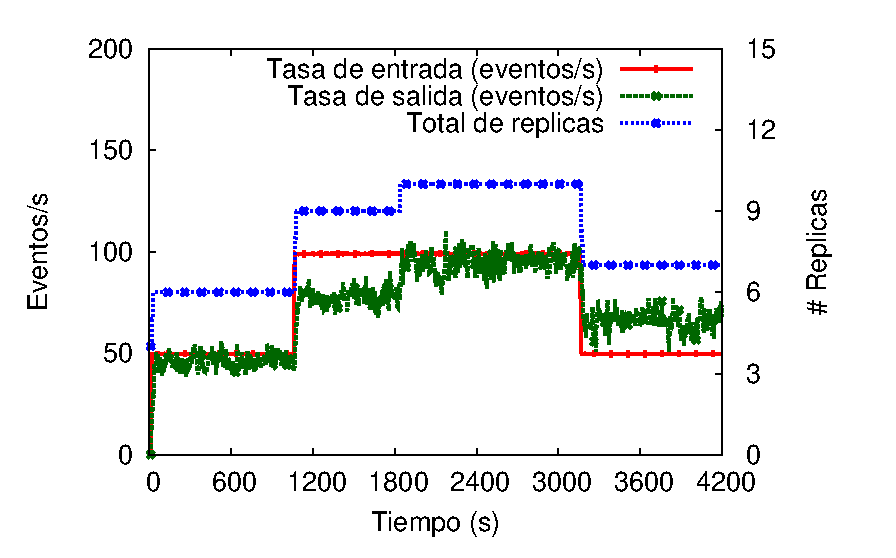
\includegraphics[scale=0.4]{images/exp/app1/normal/cm/processSystem.eps}
\end{figure}

\begin{figure}[p]
	\centering
	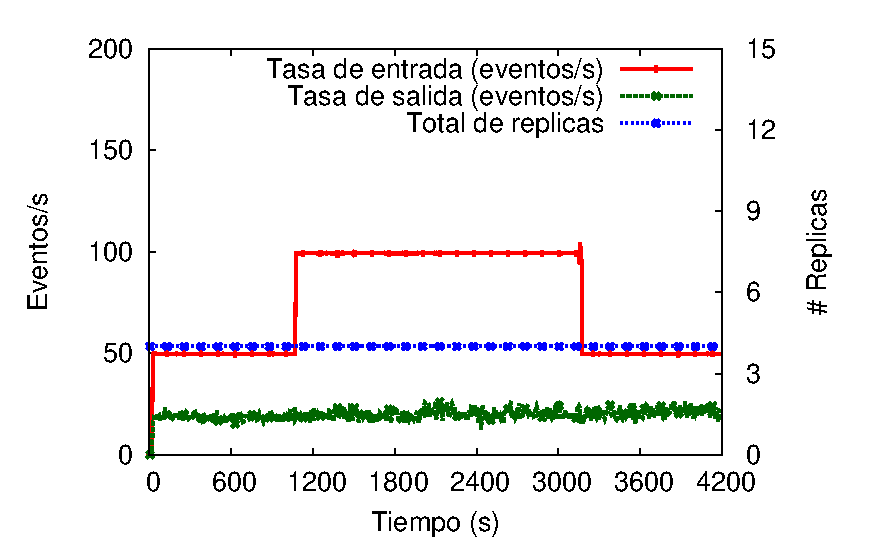
\includegraphics[scale=0.4]{images/exp/app1/normal/sm/processSystem.eps}
\end{figure}
\end{multicols}
\end{frame}

\begin{frame}{Experimentos y evaluación}{Aplicación 1 - Variable - Cantidad total de eventos procesados}

\begin{itemize}
\item 303.156 eventos procesados con uso del modelo \textit{vs} 82.770 eventos procesados sin uso del modelo
\item Mejora de 3 veces la cantidad de eventos procesados
\end{itemize}

\begin{multicols}{2}
\begin{figure}[p]
	\centering
	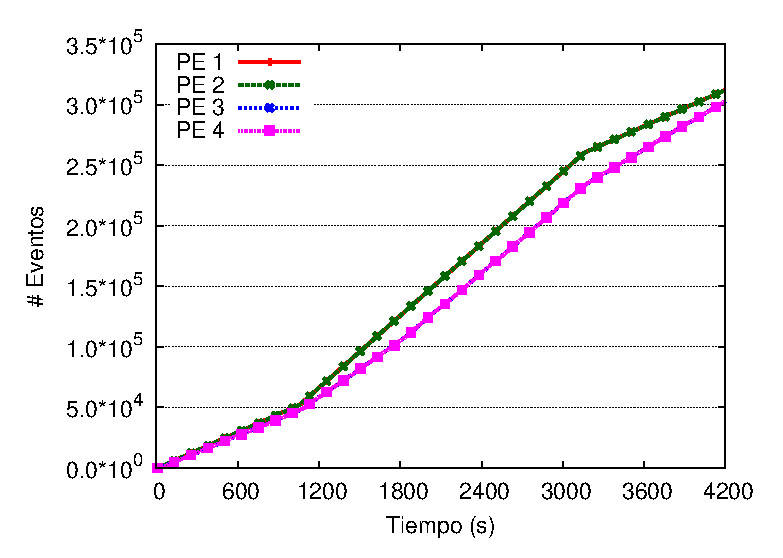
\includegraphics[scale=0.475]{images/exp/app1/normal/cm/eventCount.eps}
\end{figure}

\begin{figure}[p]
	\centering
	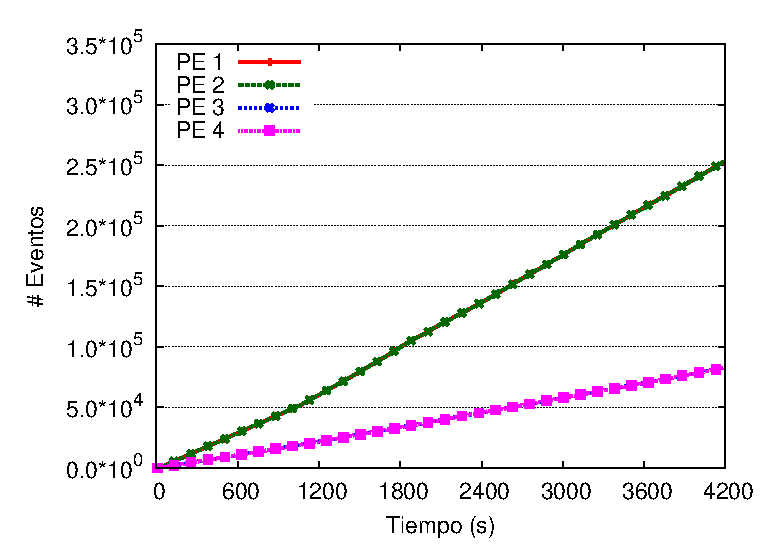
\includegraphics[scale=0.475]{images/exp/app1/normal/sm/eventCount.eps}
\end{figure}
\end{multicols}
\end{frame}

%%% App 2 - Constante %%%

\begin{frame}{Experimentos y evaluación}{Aplicación 2 - Constante - Rendimiento y cantidad de réplicas}

\begin{multicols}{2}
\begin{figure}[p]
	\centering
	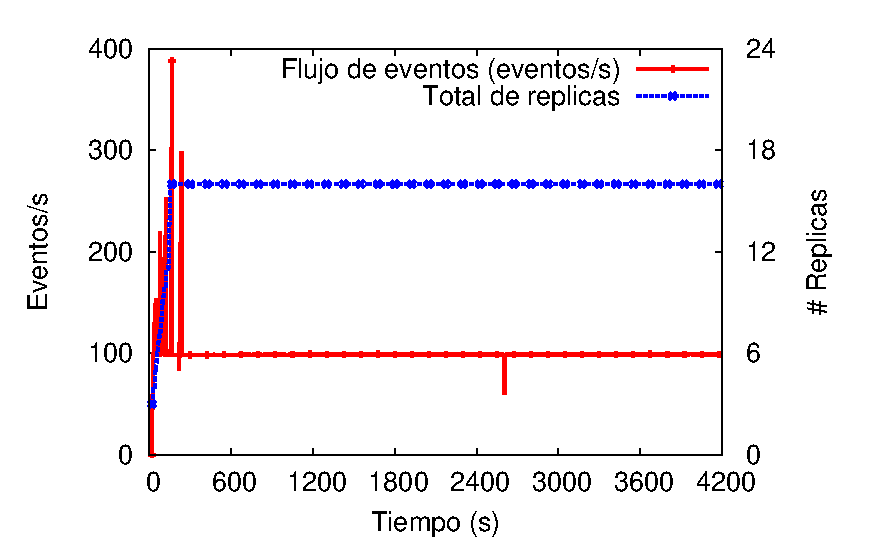
\includegraphics[scale=0.4]{images/exp/app2/uniform/cm/processSystem.eps}
\end{figure}

\begin{figure}[p]
	\centering
	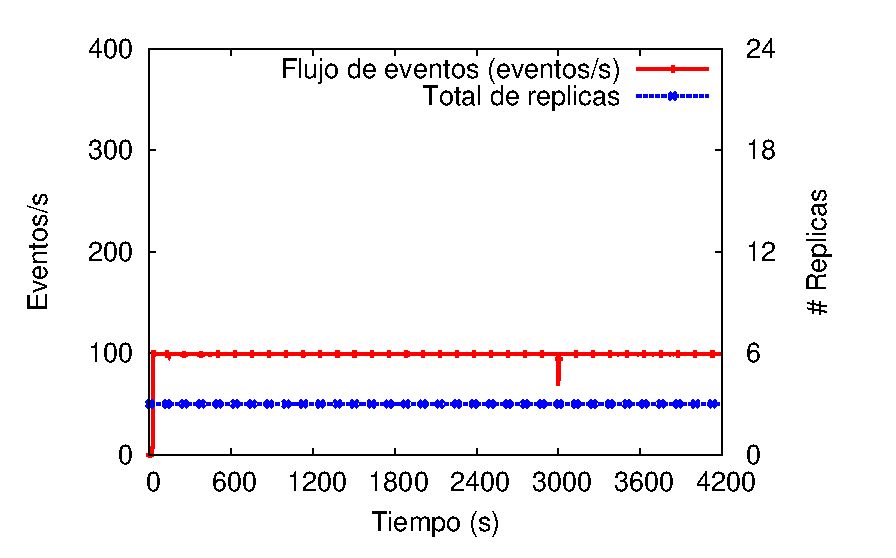
\includegraphics[scale=0.4]{images/exp/app2/uniform/sm/processSystem.eps}
\end{figure}
\end{multicols}
\end{frame}

\begin{frame}{Experimentos y evaluación}{Aplicación 2 - Constante - Cantidad total de eventos procesados}

\begin{itemize}
\item 275.290 eventos procesados con uso del modelo \textit{vs} 28.152 eventos procesados sin uso del modelo
\item Mejora de 9 veces la cantidad de eventos procesados
\end{itemize}

\begin{multicols}{2}
\begin{figure}[p]
	\centering
	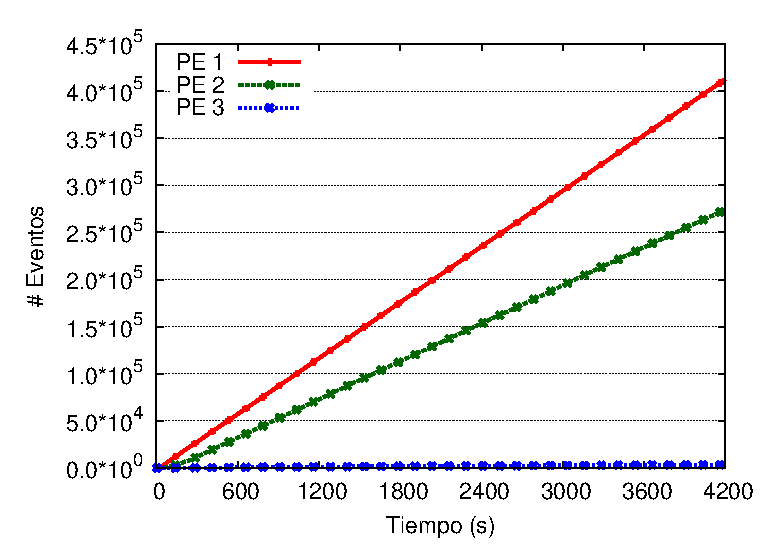
\includegraphics[scale=0.475]{images/exp/app2/uniform/cm/eventCount.eps}
\end{figure}

\begin{figure}[p]
	\centering
	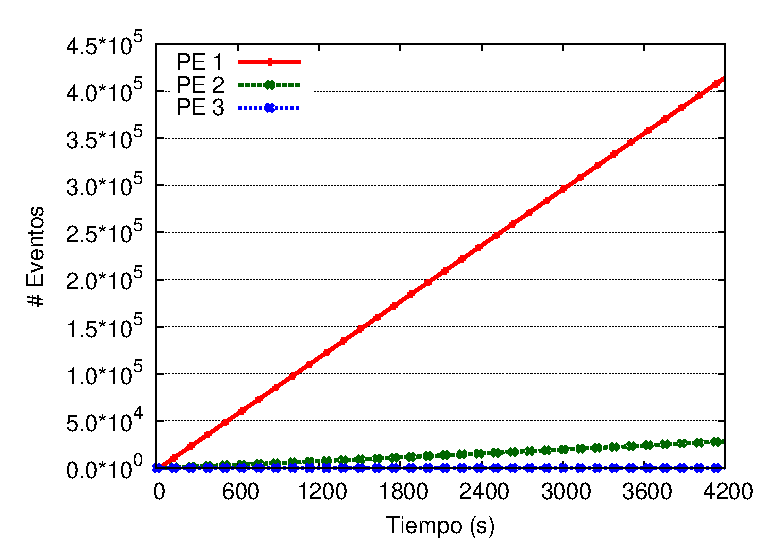
\includegraphics[scale=0.475]{images/exp/app2/uniform/sm/eventCount.eps}
\end{figure}
\end{multicols}
\end{frame}

%%% App 2 - Variable %%%

\begin{frame}{Experimentos y evaluación}{Aplicación 2 - Variable - Rendimiento y cantidad de réplicas}

\begin{multicols}{2}
\begin{figure}[p]
	\centering
	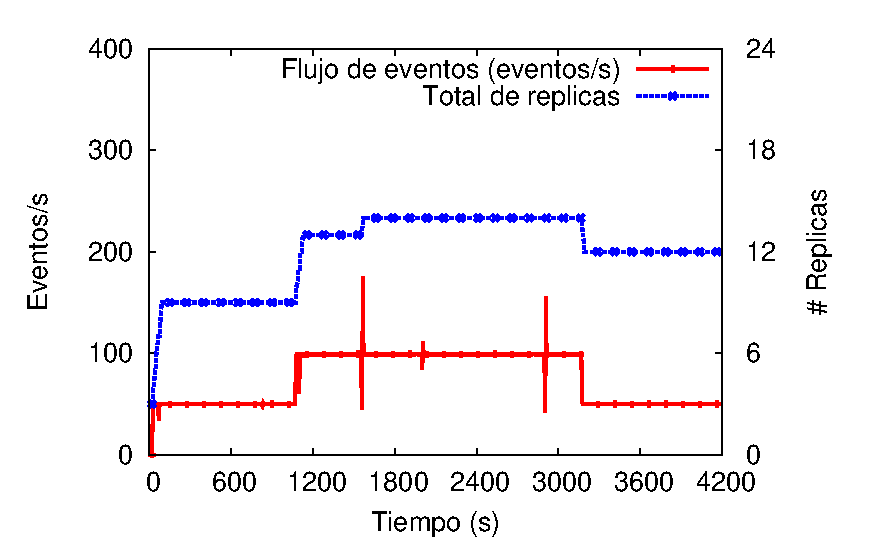
\includegraphics[scale=0.4]{images/exp/app2/normal/cm/processSystem.eps}
\end{figure}

\begin{figure}[p]
	\centering
	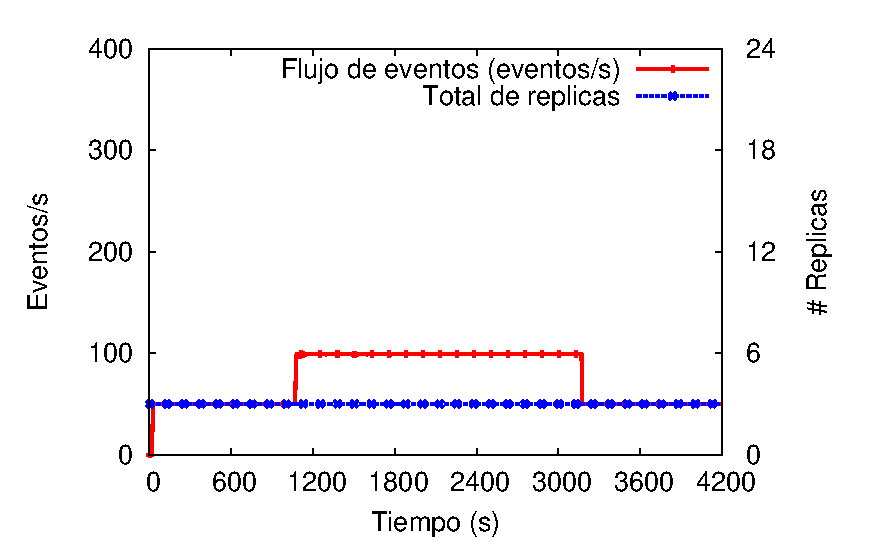
\includegraphics[scale=0.4]{images/exp/app2/normal/sm/processSystem.eps}
\end{figure}
\end{multicols}
\end{frame}

\begin{frame}{Experimentos y evaluación}{Aplicación 2 - Variable - Cantidad total de eventos procesados}

\begin{itemize}
\item 228.942 eventos procesados con uso del modelo \textit{vs} 27.751 eventos procesados sin uso del modelo
\item Mejora de 8 veces la cantidad de eventos procesados
\end{itemize}

\begin{multicols}{2}
\begin{figure}[p]
	\centering
	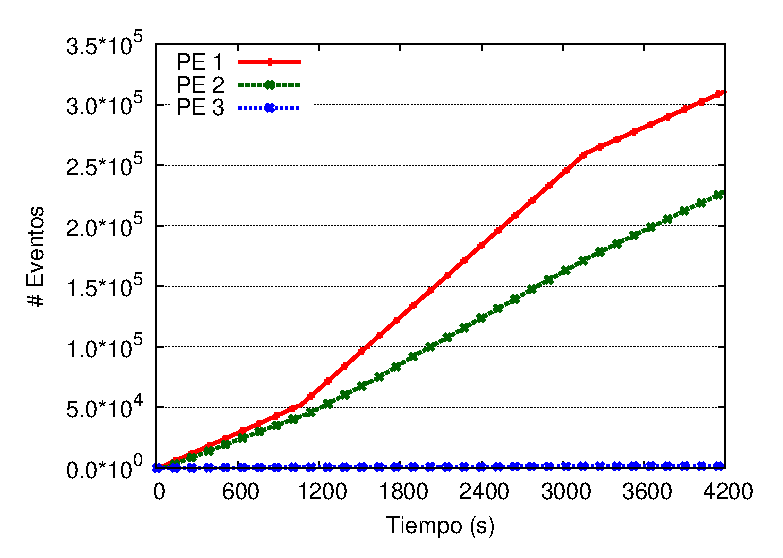
\includegraphics[scale=0.475]{images/exp/app2/normal/cm/eventCount.eps}
\end{figure}

\begin{figure}[p]
	\centering
	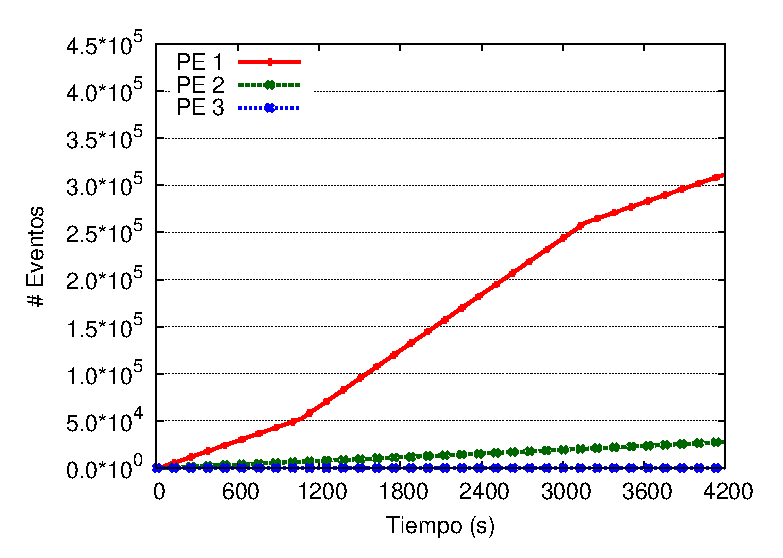
\includegraphics[scale=0.475]{images/exp/app2/normal/sm/eventCount.eps}
\end{figure}
\end{multicols}
\end{frame}

%%% Total de eventos procesados %%%

\begin{frame}{Experimentos y evaluación}{Cantidad de eventos procesados}

\begin{figure}[p]
	\centering
	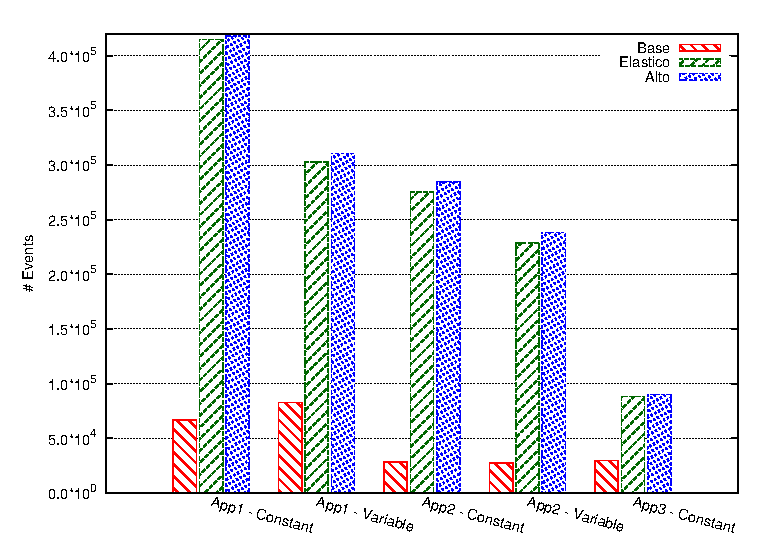
\includegraphics[scale=0.7]{images/exp/eventTotal.eps}
\end{figure}
\end{frame}